Once the user has selected properties to augment their data with, e.g. the artist biography modeled in the Smithsonian dataset with \scalebox{.6}[1]{$<$}{http://collection.americanart.si.edu/id/ontologies\#PE\_has\_note\_primaryartistbio}\scalebox{.6}[1]{$>$} and the the birth event modeled with \scalebox{.6}[1]{$<$}{http://www.cidoc-crm.org/cidoc-crm/P98i\_was\_born}\scalebox{.6}[1]{$>$}, Karma begins to pull in data from the data repository.
It does so by generating SPARQL queries.  
Karma first generates a list of URIs from the current dataset to augment to anchor the queries.  
To expand the search, the user also has the option of specifying an equivalence relationship like owl:sameAs or skos:exactMatch.  
Karma then binds a set of predicates, and classes for object properties, as indicated by the user, and then executes the queries.  
Karma finally merges the results in to the dataset and adds the appropriate links to the source model as illustrated in Figure~\ref{fig:augment-screenshot}
.  
\begin{figure*}
\begin{center}
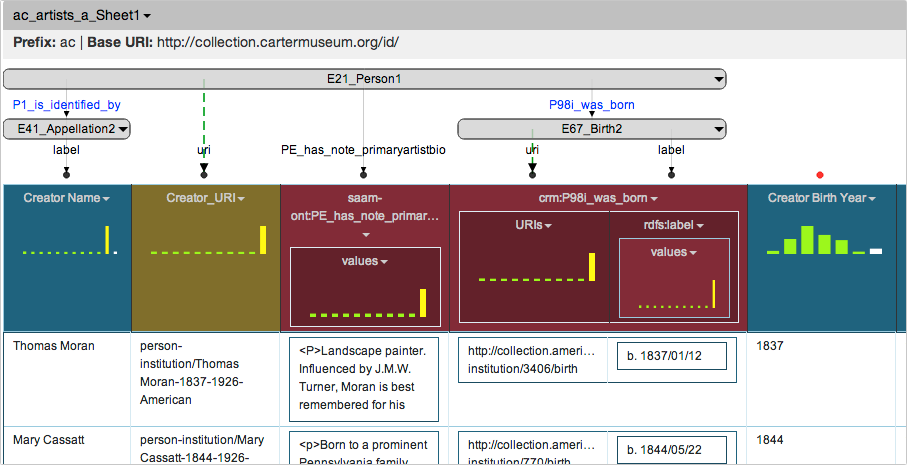
\includegraphics[width=4.9in]{images/6-augment.png}
\vspace{-3mm}
\caption{Fully integrated data from the Smithsonian sources}
\vspace{-2mm}
\label{fig:augment-screenshot}
\end{center}
\vspace{-1.5em}
\end{figure*}
